\documentclass[conference]{IEEEtran}
\usepackage{graphicx}
\usepackage[strings]{underscore}
\usepackage{biblatex}

%Title
\title{Exploring Otsu's Method}
\author{
    \IEEEauthorblockN{Sotheanith Sok}
    \IEEEauthorblockA{
        Department of Engineering\\ 
        California State University of Long Beach\\
        Sotheanith.Sok@student.csulb.edu
    }
}
\date{September 9 2021}

\addbibresource {refs.bib}

\begin{document}
\maketitle

\section{Introduction}
In computer vision, image segmentation is the process of dividing an image into multiple segments and these segments tend to simplify the image which will make it easier to analyze such image for other purposes such as boundary locating, object finding, and many more. One of the simpler types of image segmentation is splitting a gray-scale image between a foreground area and a background area by picking a pixel intensity threshold that separates the two areas. Unfortunately, picking the pixel intensity threshold manually is not efficient as any given threshold can only work for a selective group of images. Thus, a more adaptive approach is necessary and Otsu's method is one of them.

Otsu's method, named after Nobuyuki Otsu, is an algorithm for automatically determining a pixel intensity threshold that separates a background area from a foreground area of any gray-scale image. This is possible under the assumption that there is a bi-modal distribution, with each peak represents a background area or a foreground area, when examining the histogram generated from pixel intensities and pixel counts of a given image \cite{wikipedia-contributors:2020}.

\begin{figure}[!htb]
    \centering
    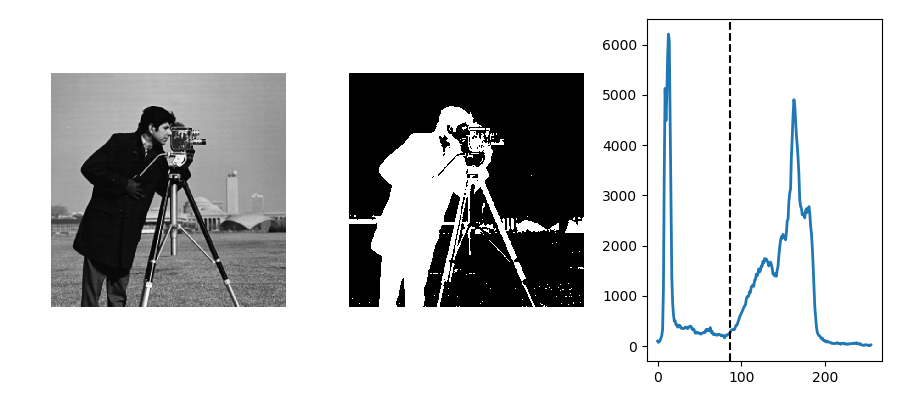
\includegraphics[width=\linewidth]{otsu_example.png}
    \caption{Original image, binary image, and histogram used or generated by Otsu's method \cite{scipy-lectures:2020}.}
\end{figure}

\section{The Algorithm}
In order to find the pixel intensity threshold, Otsu's method will perform an exhaustive search of all pixel intensity values and select a value that maximizes the inter-class variance. For any given image, the algorithm starts by generating a histogram representing all pixel intensities and the numbers of pixels that have such intensities \cite{tay:2020}. Then, according to \cite{greensted:2010}, an inter-class variance can be represented as
\[\sigma_w^2 = W_f\sigma_f^2 + W_b\sigma_b^2\]
where:
\begin{description}
    \item[$\sigma_w^2$] is the inter-class variance.
    \item[$W_f$] is the weight of the foreground area.
    \item[$\sigma_f^2$] is the variance of the foreground area.
    \item[$W_b$] is the weight of the background area.
    \item[$\sigma_b^2$] is variance of the background area.
\end{description}
. Weights of the foreground area and the background area can be calculated with the following formula
\[W_b =  \frac{\sum_{i=0}^{t-1} P(i)}{\sum_{i=0}^{all} P(i)} \]
\[W_f =  \frac{\sum_{i=t}^{all} P(i)}{\sum_{i=0}^{all} P(i)} \]
where:
\begin{description}
    \item[$W_b$] is the weight of the background area.
    \item[$W_f$] is the weight of the foreground area.
    \item[$t$] is the pixel intensity threshold.
    \item[$P(i)$] is the pixel count at intensity $i$.
\end{description}
The remaining factors, which are variances of both the background area and the foreground area, can be calculated from the mean of each area respectively with the following formula
\[\mu_b = \frac{\sum_{i=0}^{t-1} i P(i)}{\sum_{i=0}^{t-1}P(i)}\]
\[\sigma_b^2 = \frac{\sum_{i=0}^{t-1}(i-\mu_b)^2 \times P(i)}{\sum_{i=0}^{t-1}P(i)}\]
\[\mu_f = \frac{\sum_{i=t}^{all} i P(i)}{\sum_{i=t}^{all}P(i)}\]
\[\sigma_f^2 = \frac{\sum_{i=t}^{all}(i-\mu_f)^2 \times P(i)}{\sum_{i=t}^{all}P(i)}\]
where:
\begin{description}
    \item[$\mu_b$]is the mean of the background area.
    \item[$\mu_f$]is the mean of the foreground area.
    \item[$\sigma_b^2$] is the variance of the background area.
    \item[$\sigma_f^2$] is the variance of the foreground area.
    \item[$t$] is the intensity threshold.
    \item[$P(i)$] is the pixel count at $i$ intensity.
\end{description}
The entire process is repeated for all pixel intensities and the one that produces the largest inter-class variance will be picked as the final pixel intensity threshold.

\section{Limitation}
While Otsu's method performs well on most gray-scale images, it still has some problems when processing images that do not produce the bi-modal distribution with high peaks and deep valleys \cite{kang-and-atul:2019}.
\begin{figure}[!htb]
    \centering
    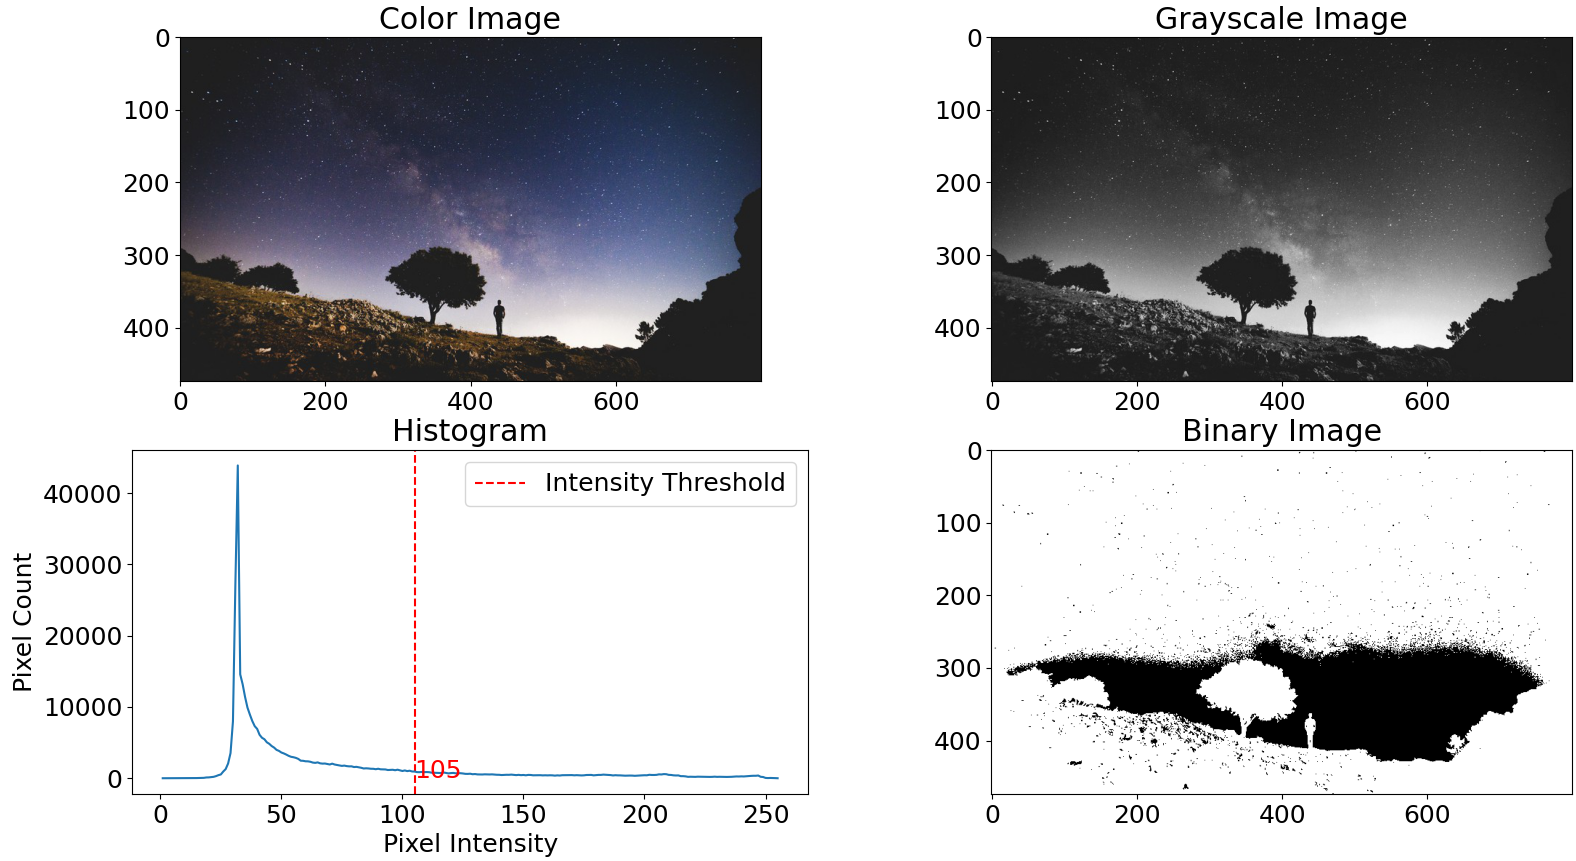
\includegraphics[width=\linewidth]{small_object_image.png}
    \caption{Otsu's method performance on an image with a small foreground area \cite{altphotos:2017}.}
\end{figure}
To start with, any image that has a foreground area significantly smaller than a background area tends to not do well with Otsu's method due to the lack of pixels count in a foreground area which is often necessary for generating a high peak in the image's histogram.
\begin{figure}[!htb]
    \centering
    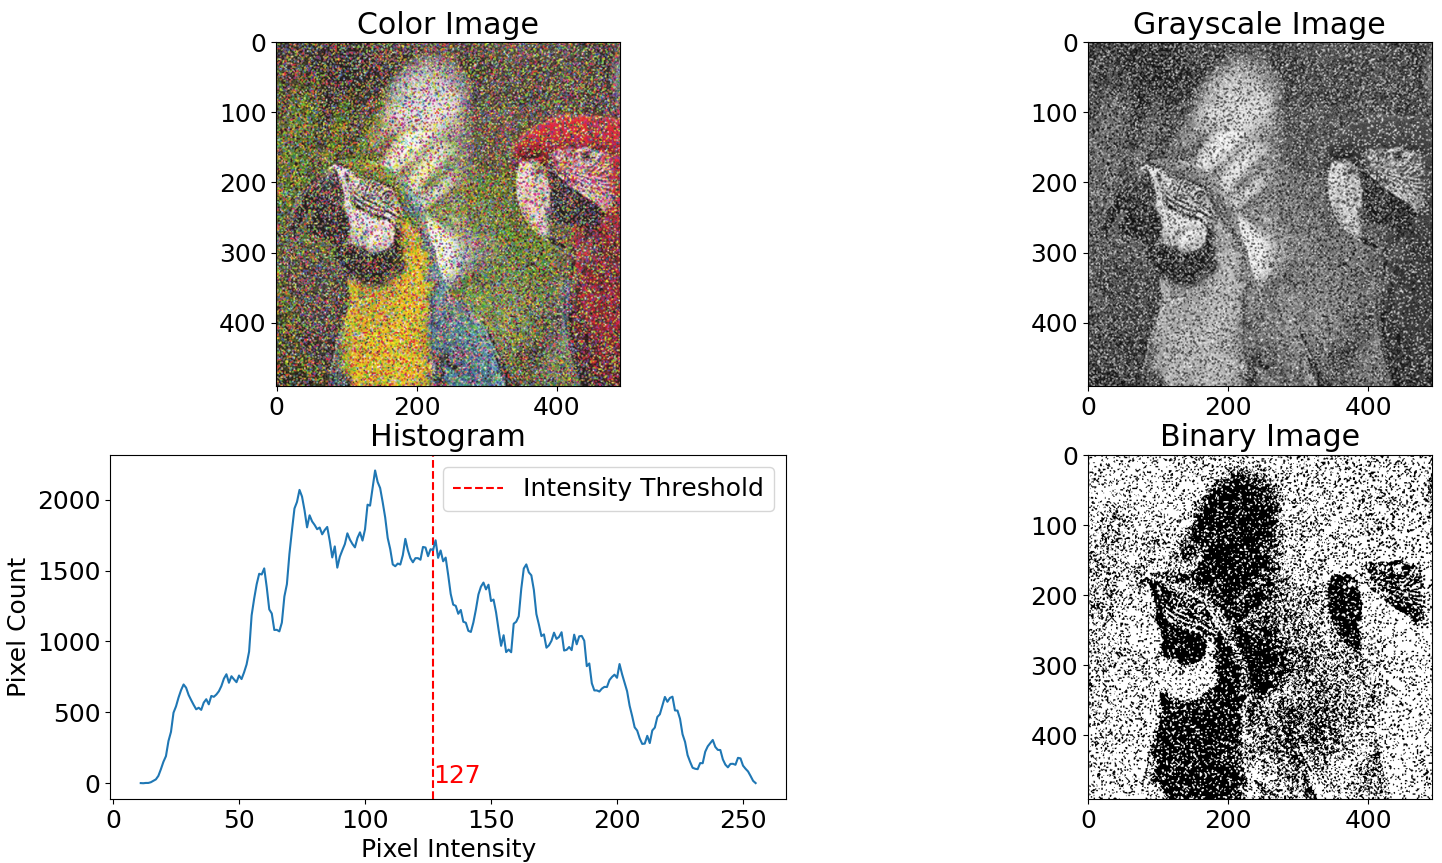
\includegraphics[width=\linewidth, scale=1.5]{noisy_image.png}
    \caption{Otsu's method performance on an image that contains a lot of noise \cite{qrcode:2012}.}
\end{figure}
Then, there are images with a lot of noise. This type of image also does not perform well with Otsu's method because noises in such images often prohibit the formation of bi-modal distribution in the histogram.
\begin{figure}[!htb]
    \centering
    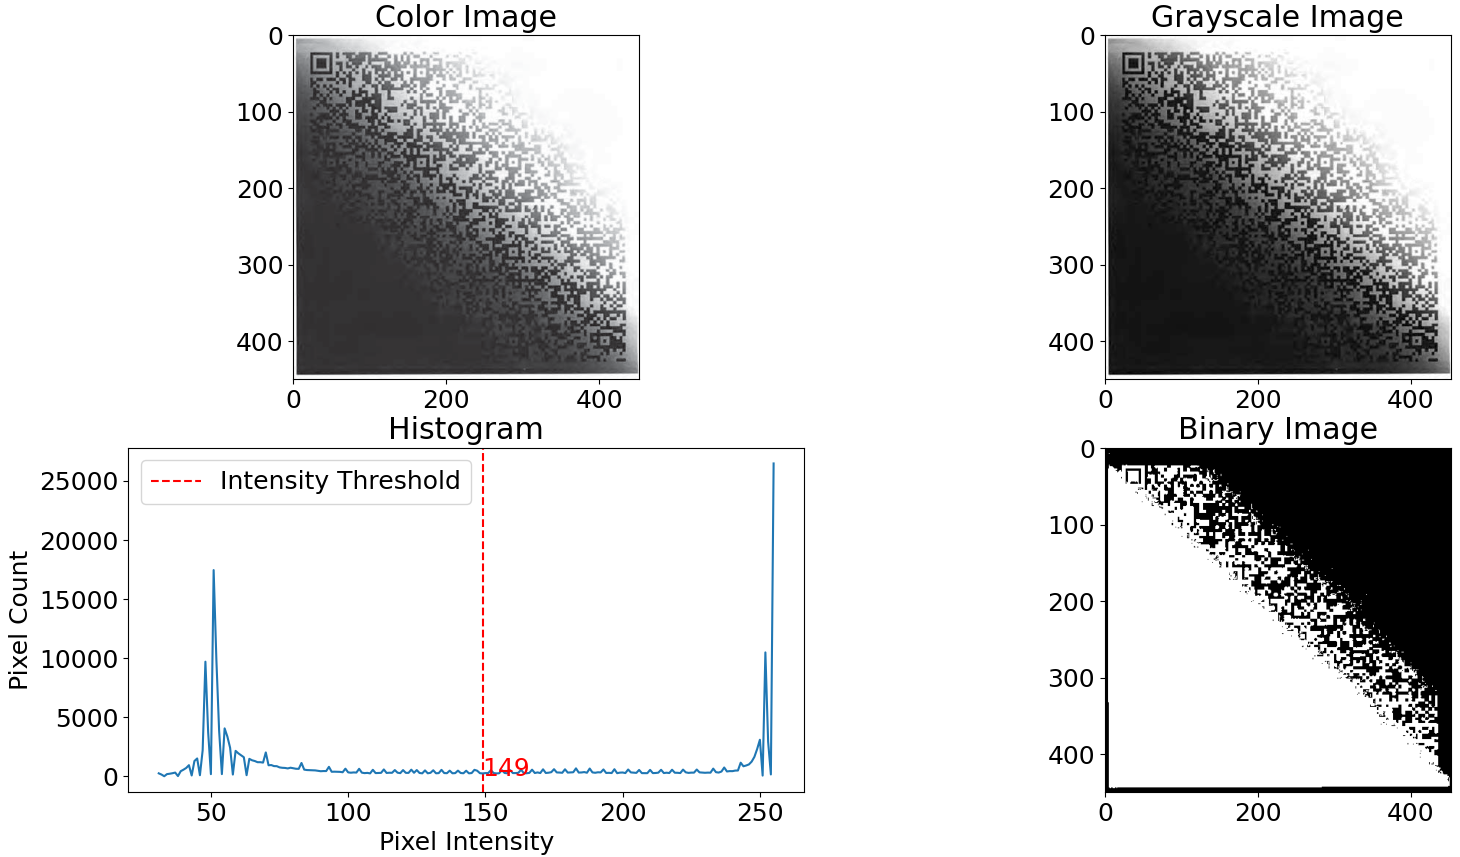
\includegraphics[width=\linewidth]{non-uniform illumination_image.png}
    \caption{Otsu's method performance on an image with non-uniform illumination \cite{bird:2014}.}
\end{figure}
Last but not least, the Otsu's method performs poorly on images with non-uniform illumination because it uses a single global threshold to separate the background area and the foreground area. To simply put, for such an image, a section of the background area might have the same illumination as another section of the foreground area and vice versa.

\section{Final Thought}
Otsu' method is a great choice for finding a global intensity threshold for splitting a gray-scale image into a foreground area and a background area. However, due to the nature of the algorithm which relies heavily on an image's intensities having a bi-modal distribution, it should not be applied universally to all gray-scale images. To overcome the limitations of Otsu's method, preprocessing techniques such as image denoising and others should be used before applying Otsu' method onto an image.

\printbibliography

\end{document}
